%%%%%%%%%%%%%%%%%%%%%%%%%%%%%%%%%%%%%%%%%%%%%%%%%%%%%%%%%%%%%%%%%%
%%%
%%%       CONCOURS CNAP  - FICHE RECAPITULATIVE.
%%% 
%%%     Version 7.12.2016 -  % Editer par Olga Alexandrova et Kevin Belkacem
%%%     
%%%%%%%%%%%%%%%%%%%%%%%%%%%%%%%%%%%%%%%%%%%%%%%%%%%%%%%%%%%%%%%%%%

\documentclass[11pt]{article}
\usepackage[pdftex]{graphicx}
\usepackage{amsmath}
\usepackage[pdftex]{hyperref}
\hypersetup{
    colorlinks,%
    citecolor=black,%
    filecolor=black,%
    linkcolor=black,%
    urlcolor=blue     % can put red here to visualize the links
}
\oddsidemargin=0.2cm
\topmargin=-1.5cm
\textwidth=16cm
\textheight=25cm
\pagestyle{empty}
\voffset -1cm
\parindent 0pt
\begin{document}
\begin{center}
\textbf {CONCOURS ASTRONOME-ADJOINT 2017 -- FICHE R\'ECAPITULATIVE}\\ 
\vspace{0.2cm}


\hrule
\end{center}

%%%%%%%%%%%%%%%%%%%%%%%%%%%%%%%%%%%%%%%%%%%%%%%%%%%%%%%%%%%%%%%%%%%%%%%%%%%

\begin{minipage}{11cm}

\vspace{0.2cm}

{\bf NOM, Pr\'enom :} EL MELLAH, Ileyk\\
{\bf Date de naissance :} 5 Avril 1989 \\
{\bf Nombre de candidatures ant\'erieures :} 0 \\
{\bf Interruption(s) d'activit\'e(s) :}  - 

\vspace{0.1cm}

{\bf \'Etablissement et \'equipe d'accueil demand\'es :}\\
Observatoire de Paris \rule[-0.4ex]{0.2ex}{1.2em} Laboratoire de l'Univers et des ses Th\'eories\\ Equipe \textit{Ph\'enom\`enes aux Hautes Energies}


%%%%%%%%%%%%%%%%%%%%%%%%%%%%%%%%%%%%%%%%%%%%%%%%%%%%%%%%%%%%%%%%%%%%%%%%%%%


\end{minipage}  
\hspace{1.5cm}
\begin{minipage}{4cm}
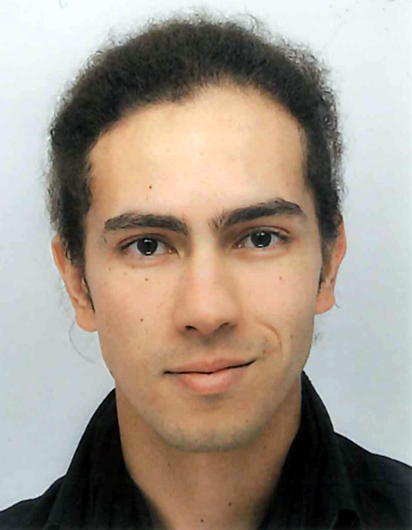
\includegraphics[height=4.cm] {ID_photo.png}
\end{minipage}

%%%%%%%%%%%%%%%%%%%%%%%%%%%%%%%%%%%%%%%%%%%%%%%%%%%%%%%%%%%%%%%%%%%%%%%%%


\vspace{0cm}
{\bf Post-doctorats et situation actuelle :}\\
Mai 2017 - Juin 2020 \rule[-0.4ex]{0.2ex}{1.2em} Bourse FWO $[$Pegasus$]^2$ Marie Sk\l{}odowska-Curie \rule[-0.4ex]{0.2ex}{1.2em} 3 ans \rule[-0.4ex]{0.2ex}{1.2em} KU Leuven\\
Octobre 2016 - Mai 2017 \rule[-0.4ex]{0.2ex}{1.2em} Contrat postdoctoral \rule[-0.4ex]{0.2ex}{1.2em} 8 mois \rule[-0.4ex]{0.2ex}{1.2em} KU Leuven\\

\vspace{-0.2cm}
{\bf Th\`ese :} \textit{Wind accretion onto compact objects}, supervis\'e par Fabien Casse \& Andrea Goldwurm au laboratoire AstroParticule \& Cosmologie de Paris 7 (\'equipe \textit{Astrophysique des hautes \'energies}). Soutenance le 7 Septembre 2016 (apr\`es 3 ans). 


%%%%%%%%%%%%%%%%%%%%%%%%%%%%%%%%%%%%%%%%%%%%%%%%%%%%%%%%%%%%%%%%%%%%%%%%%
%%%                RECHERCHE :

\vspace{0.2cm}
{\bf Th\`emes des recherches effectu\'ees : } Stellar remnant : neutron star (NS), black hole (BH), white dwarf (WD) - Accretion : Roche lobe overflow, wind accretion - Binary system : X-ray binary (XB), Cataclysmic variable (CV) - Stellar outflow : line-driven wind

%\emph{D\'esignez  avec quelques mots clefs repr\'esentatifs votre domaine de recherche} 
%I model mass transfer in binary systems hosting a star and a stellar remnant (compact object or white dwarf), i.e. in X-ray binaries and Cataclysmic variables. It proceeds either via Roche lobe overflow or through the stellar wind. A fraction of the latter can be captured by the compact object in Supergiant X-ray binaries such as Vela X-1. As the flow is accreted, it emits copious amounts of light whose photometric and spectroscopic time-variability suggests structures in the flow I try to identify with numerical simulations of these systems.

\vspace{0.3cm}

%%%%%%%%%%%%%%%%%%%%%%%%%%%%%%%%%%%%%%%%%%%%%%%%%%%%%%%%%%%%%%%%%%%%%%%%%
%%%  METHODOLOGIE :

{\bf M\'ethodologies :}  
Th\'eorie --  Mod\'elisation -- Simulations

\vspace{0.3cm}

{\bf T\^{a}ches de service effectu\'ees et/ou envisag\'ees :}\\
%\emph{ Pr\'ecisez le titre, le service d'observation (ANO1 \`a ANO6), le responsable national et d\'ecrivez succinctement l'activit\'e}
ANO5 - Eric Slezak - With Franck Le Petit and Jacques Le Bourlot at the LERMA, reduction of maps of the Interstellar Medium using the Meudon PDR code. With the MIS and Jets platform, confront observations to models with optimization and inverse problems techniques.\\

\vspace{-0.1cm}

{\bf Enseignements effectu\'es :}\\
\makebox[1.5cm][l]{2016-17} \makebox[7cm][l]{Computational methods for Astrophysics} \makebox[2.5cm][l]{60h TD} \makebox[1.5cm][l]{5$^{\text{th}}$ year} \makebox[3.5cm][l]{KU Leuven}\\
\makebox[1.5cm][l]{2014-16} \makebox[7cm][l]{Classical Mechanics} \makebox[2.5cm][l]{128h TD} \makebox[1.5cm][l]{1$^{\text{st}}$ year} \makebox[3.5cm][l]{Paris 7}\\ 
\makebox[1.5cm][l]{2013} \makebox[7cm][l]{Physics for Medical studies} \makebox[2.5cm][l]{32h TD} \makebox[1.5cm][l]{1$^{\text{st}}$ year} \makebox[3.5cm][l]{Paris 7}\\ 
\makebox[1.5cm][l]{2013} \makebox[7cm][l]{Deterministic systems and signals} \makebox[2.5cm][l]{32h TP} \makebox[1.5cm][l]{4$^{\text{th}}$ year} \makebox[3.5cm][l]{Paris 7}\\ 
%\makebox[1.5cm][l]{2012-13} \makebox[7cm][l]{Private lessons with the company \emph{Cours Thal\`es}}- Paris\\ 
\makebox[1.5cm][l]{2009-10} \makebox[6.9cm][l]{Teaching assistant} \makebox[2.5cm][l]{16h CM-TP} \makebox[4.5cm][l]{high school Gustave Eiffel}\\ 

\vspace{-0.1cm}

{\bf R\'esultats principaux :} \\
%\emph{D\'ecrivez de mani\`ere synth\'etique ceux de vos r\'esultats qui vous paraissent les plus pertinents }
\underline{2017:} impact of inhomogeneities in the wind of Supergiant (Sg) stars on the time-variability of accretion and absorption in SgXB. Confrontation to observations of Vela X-1 with Chandra. \underline{2016:} orbital shearing of the stellar wind in SgXB and formation of wind-capture discs. \underline{2015:} accretion of a supersonic planar uniform flow by a compact object (structure of the bow shock, quantification of the mass accretion rate, topology of the inner sonic surface).\\

\vspace{-0.1cm}

{\bf Programme de recherche :}  
\underline{1.} Evaluation of the impact of the magnetic field of the NS or WD on the innermost regions of the accreted flow in SgXB and CV. Synthetic observations and confrontation to observations of Vela X-1 and to the intermediate polar CV V4743 Sgr. \underline{2.} Accretion of a low angular momentum flow onto a BH to determine whether there might be a disc-like structure lying near the last stable orbit. Comparisons to observations of Sgr A* by GRAVITY and the EHT, using the ray-tracing code GYOTO to produce synthetic observations.\\

\vspace{-0.1cm}

{\bf Comp\'etences acquises et points forts de votre candidature :}  
Wide expertise in Computational Astrophysics. Improvements of \href{http://amrvac.org/}{\texttt{MPI-AMRVAC}}, a finite volume code to numerically solve the equations of MHD, on an adaptive grid whose geometry can be adapted to the needs of a physical problem. I also gained experience in adjacent domains such as visualization, high performance computing, hardware, cluster and data management, profiling and code optimization.

\newpage

%%%%%%%%%%%%%%%%%%%%%%%%%%%%%%%%%%%%%%%%%%%%%%%%%%%%%%%%%%%%%%%%%%%%%%%%%

\section*{Publications}
\vspace{0.3cm}


{\bf Nombre de publications de rang A publi\'ees et sous presse:} 8 \\
 
{\bf Nombre de publications de rang A soumises:} 0 \\

{\bf Nombre de communications et/ou de posters pr\'esent\'es \`a des
  conf\'erences:} 11 \\
  
{\bf Autres (participation \`a des ouvrages, rapports techniques, codes, logiciels, sites web, etc...) :}\\ \\
\makebox[1cm][l]{2017} Radio show \href{https://www.mixcloud.com/faconde/faconde-s2e01-vulgarisation/}{\emph{Faconde}} on scientific outreach (Radio Campus, Bruxelles)\\ \\
\makebox[1cm][l]{2016} \href{http://adsabs.harvard.edu/abs/2017arXiv170709165E}{PhD manuscript}\\ \\
\makebox[1cm][l]{2015} Festival of Sciences (Paris 7) and 3D-printing of Roche potentials \\ \\
\makebox[1cm][l]{2015} \href{http://homes.esat.kuleuven.be/~ileyk}{Personal webpage}\\ \\
\makebox[1cm][l]{2015} \href{http://rjp.sfp-paris.fr/index2015.html}{Website of the \emph{Rencontres des Jeunes Physiciens 2015}}\\ \\
\makebox[1cm][l]{2015} Community manager of the \emph{Rencontres des Jeunes Physiciens 2015}\\ \\
\makebox[1cm][l]{2015} Wolfram demonstration \href{http://demonstrations.wolfram.com/TrajectoryOfATestMassInARochePotential/}{\textit{Trajectory of a Test Mass in a Roche Potential}}\\
\vspace{0.3cm}


{\bf Liste des 5 publications de rang A, par ordre d'importance, qui illustrent le mieux votre travail et vos comp\'etences   (avec liens) :}\\ \\
\href{http://adsabs.harvard.edu/abs/2017arXiv171108709E}{[1]} \textbf{El Mellah I.}, Sundqvist J. O. \& Keppens R.\\ 
\emph{Accretion from a clumpy massive-star wind in Supergiant X-ray binaries} (2017) - MNRAS\\ \\
\href{http://adsabs.harvard.edu/abs/2015MNRAS.454.2657E}{[2]} \textbf{El Mellah I.} \& Casse F. \\ 
\emph{A numerical simulations of axisymmetric hydrodynamical Bondi-Hoyle accretion}\\
\emph{on to a compact object} (2015) - MNRAS\\ \\
\href{http://adsabs.harvard.edu/abs/2017MNRAS.467.2585E}{[3]} \textbf{El Mellah I.} \& Casse F. \\ 
\emph{A numerical investigation of wind accretion in persistent Supergiant X-ray Binaries}\\
\emph{I - Structure of the flow at the orbital scale} (2016) - MNRAS\\ \\
\href{http://adsabs.harvard.edu/abs/2017arXiv171106743G}{[4]} Grinberg V., Hell N., \textbf{El Mellah I.}, Neilsen J., Sander A. A. C., Leutenegger M. A.,\\
F\"{u}rst F., Huenemoerder D. P., Kretschmar P., K\"{u}hnel M., Mart\'{i}nez-N\'{u}\~{n}ez S.,\\
Niu S., Pottschmidt K., Schulz N. S., Wilms J. \& Nowak M. A.\\ 
\emph{The clumpy absorber in the high mass X-ray binary Vela X-1} (2017) - A\&A\\ \\
\href{http://adsabs.harvard.edu/abs/2017arXiv171006140X}{[5]} Xia C., Teunissen J., \textbf{El Mellah I.}, Chan\'{e} E. \& Keppens R.\\ 
\emph{MPI-AMRVAC 2.0 for solar and astrophysical applications} (2017) - ApJS\\ 


\end{document}
